\documentclass[titlepage,11pt,a4paper]{article}

\usepackage{polytechnique}
\usepackage{siunitx}
\usepackage[utf8]{inputenc}
\usepackage[frenchb]{babel}

\title{Rapport de MODAL}
\subtitle{Comment faire suivre les murs à un drone}

\author{Basile \textsc{Bruneau}\\
Youssef \textsc{Achari-Berrada}}

\date{Juin 2015}

\begin{document}
\maketitle

%Plan du rapport de MODAL

%Connexion au drone
%Application de l'algorithme lk_tracks au flux vidéo
%Présentation de la stratégie
%Réalisation de plusieurs expériences pour mesurer les vitesses des points (?> courbes, 2D, 3D)
%Régression polynomiale et obtention d'une courbe " théorique "
%Utilisation de cette courbe pour ajuster la trajectoire du drone (algorithme péchu ?> en cours)
%Difficultés, problèmes avec cet algo
%Résultats obtenus


\section{Stratégie}
L'AR.Drone disposant de peu de capteurs (pas de GPS, pas de caméra de profondeur) le seul que nous pouvions utiliser pour réaliser ce projet est la caméra frontale. C'est uniquement à partir de cet unique flux vidéo que nous avons essayé de faire suivre les murs au drone.

L'objectif étant de déplacer le drone, c'est le mouvement ici qui nous intéresse. Nous avons donc décidé d'utiliser le flux optique pour obtenir le mouvement des points de l'image. Nous avons initialement repris l'algorithme lkTracks qui calcule uniquement le mouvement des coins détectés dans l'image (ce qui permet un traitement rapide, contrairement à un calcul du mouvement de tous les points de l'image). Comme nous le verrons plus tard, l'inconvénient est que les situation où aucun coin n'est détecté dans l'image ne sont pas rares.

Ensuite l'observation importante est que lorsque le robot vole et avance en longeant un mur à sa droite (en regardant devant lui) alors les points de l'image les plus à droite ont une vitesse horizontale plus élevée que les points qui sont plus vers le centre de l'image. Et lorsque le drone avance à vitesse constante, le profil des vitesses horizontales doit probablement rester constant : les points à droite auront toujours la même vitesse, et ceux plus vers le centre également. Nous avons donc essayé de trouver ce profil des vitesses lorsque le drone longe un mur à une certaine vitesse, et ensuite en comparant la vitesse des points avec le profil théorique, nous allons essayer de corriger la trajectoire du robot.

Nous avons donc posé l'AR.Drone sur un TurtleBot que nous avons fait progressé en ligne droite le long d'un mur. Puis nous avons enregistré toutes les vitesses des points détectés par la caméra du drone. Afin d'avoir un maximum d'informations, nous avons ajouté des coins nous même sur le mur. Nous avons répété l'expérience une dizaine de fois, ce qui nous a permis d'obtenir les vitesses d'environ \num{25000} points.

Voici les résultats de ces mesures :

\begin{figure}[h]
	\caption{\label{vitesses-2d} Vitesse horizontale en fonction de la coordonnée horizontale}
	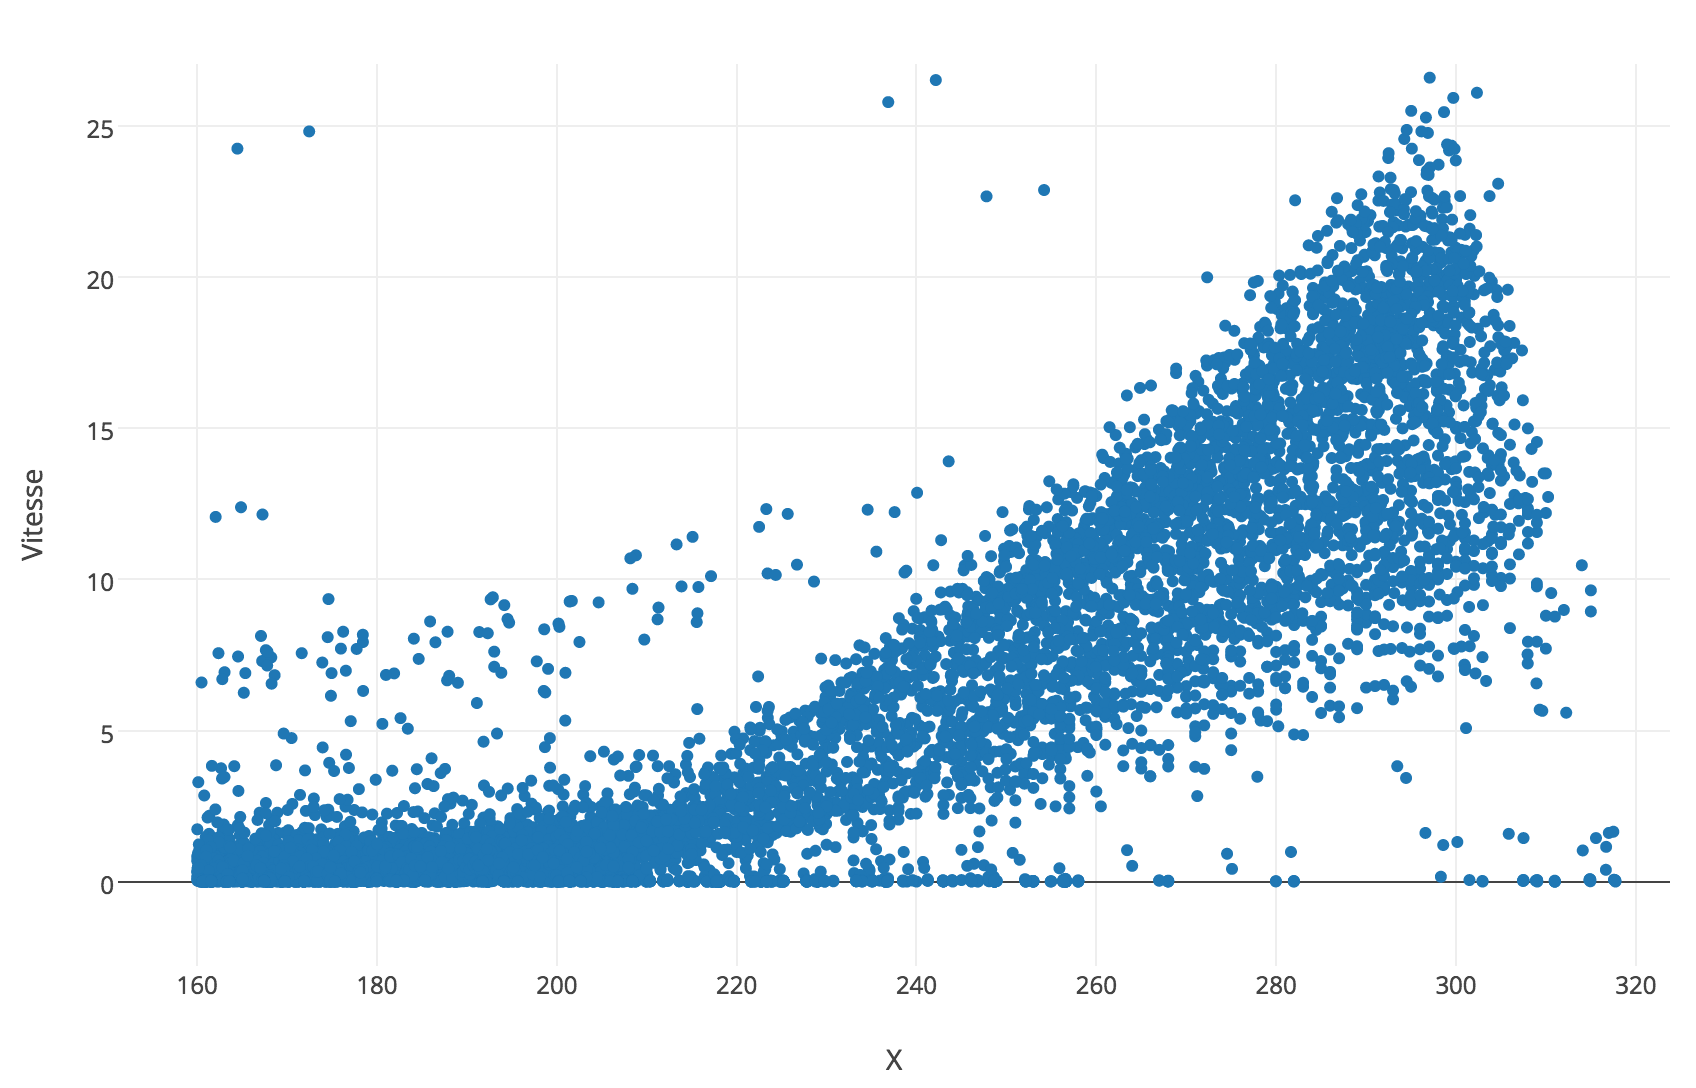
\includegraphics[scale=0.45]{images/vitesses-2d.png}
\end{figure}

On voit déjà que la vitesse horizontale au centre de l'image est quasiment nulle et qu'elle augmente plus on va vers la droite, ce qui confirme bien notre idée initiale. Nous nous sommes ensuite demandés si la coordonnée verticale avait aussi une importance.

\begin{figure}[h]
	\caption{\label{vitesses-3d-apercu} Vitesse horizontale en fonction de x et y}
	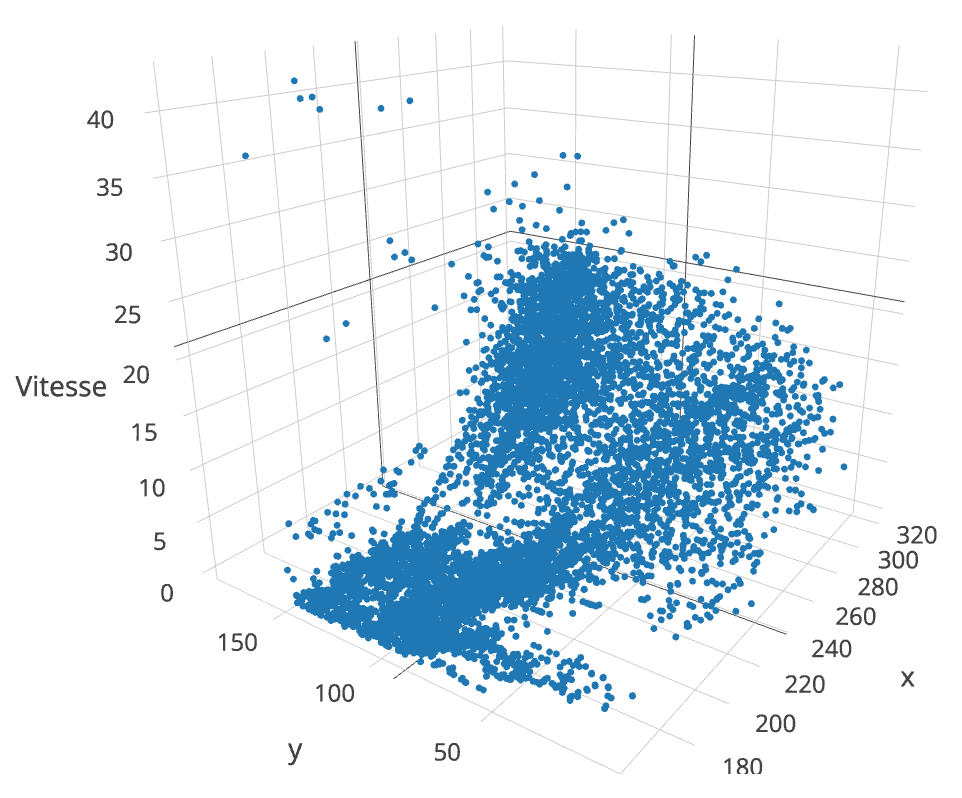
\includegraphics[scale=0.45]{images/vitesses-3d-apercu.png}
	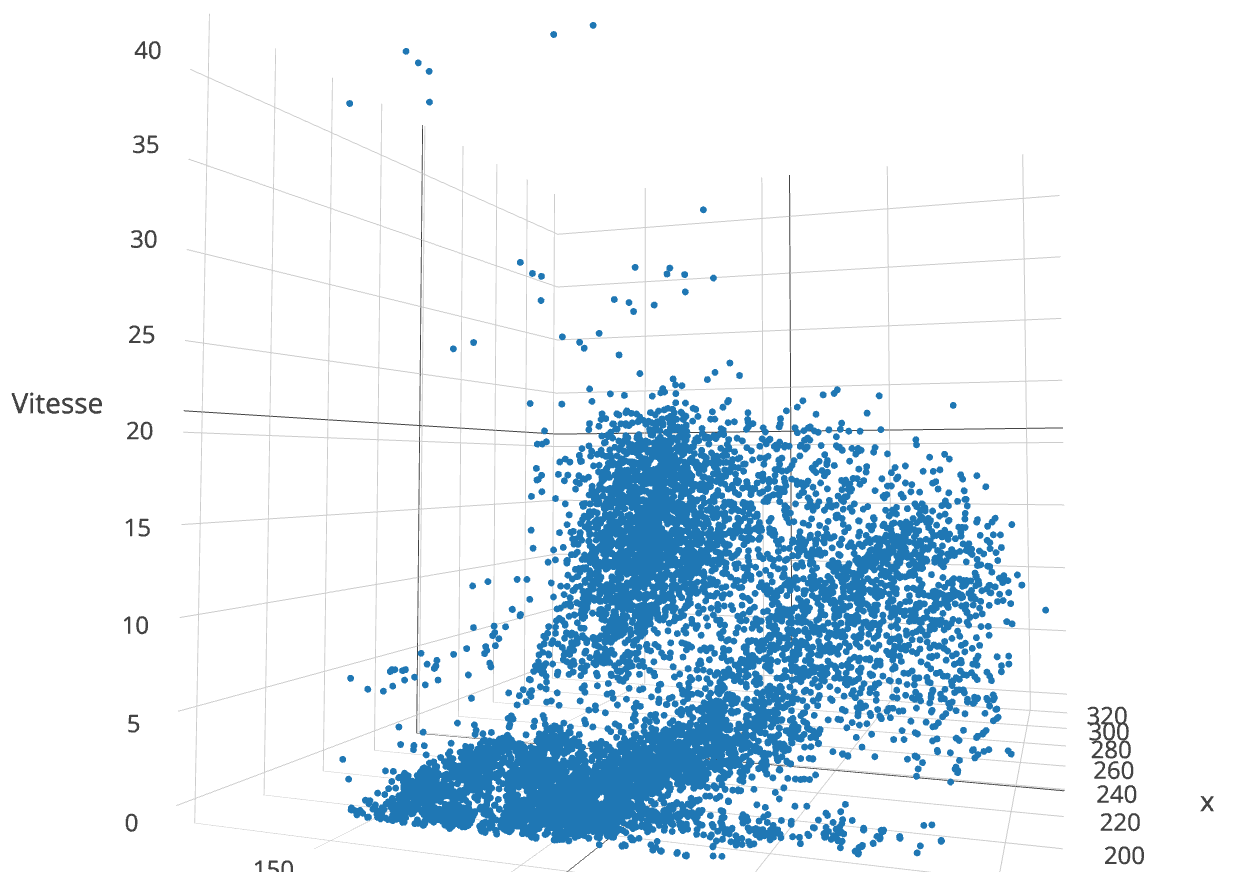
\includegraphics[scale=0.45]{images/vitesses-3d-selon-y.png}
\end{figure}

Il semble alors que la coordonnée y a une importance, les points en haut de l'image vont moins vite que ceux qui sont en bas.

\end{document}